\documentclass{article}

\usepackage[utf8]{inputenc}
\usepackage{amsmath}
\usepackage{graphicx}
\usepackage[most]{tcolorbox}
\usepackage{hyperref}


\hypersetup{
    colorlinks=true,      
    linkcolor=black,        
    citecolor=blue,        
    urlcolor=blue,         
    pdfborder={0 0 0},     
}

\title{Statistical Physics}
\author{Sabattini Manginella Cesare}
\date{December 2024}

\begin{document}

\maketitle

\tableofcontents

\newpage

\section{Introduction}
ATTENZIONE: formulario ancora in fase di sviluppo. Alcune informazioni potrebbero essere incomplete o errate.
E' inoltre in corso la riscrittura in inglese.

\newpage

\section{Micro and Macrostates}
A macrostate is the state of a system, emerging from different microscopical configurations, namely microstates.
The number of microstates corrisponding to a macrostate is called multiplicity $\Omega$.

\subsection{Entropy}
Statistically, the entropy aims to measure the degree of "ignorance" about the microscopical state of a thermodynamical system.
The formula of the S($\Omega$) function can be deduced stating the following properties:

\begin{itemize}
    \item S(1)=0.
    \item $\Omega_1>\Omega_2$ $\Longrightarrow$ $S(\Omega_1)>S(\Omega_2)$.
    \item $\Omega=\Omega_1\Omega_2$ $\Longrightarrow$ S($\Omega$)=S($\Omega_1$)+S($\Omega_2$).
\end{itemize}

Hence, ultimately, one can find the expression of the entropy for a macrostate from:

\begin{tcolorbox}[colframe=gray!50, colback=gray!10, coltitle=black, title=Boltzmann Entropy]
    Given a set of equiprobable configurations, the Boltzmann entropy can be defined from the partition function $\Omega$:
    \begin{equation}
        S = k \log \Omega
    \end{equation}
\end{tcolorbox}

\textbf{Proof:}

\begin{center}
    \begin{align*}
         & \left\{
        \begin{aligned}
             & \frac{\partial \sigma(xy)}{\partial x}=\frac{d}{dx}\sigma(x) \\
             & \frac{\partial \sigma(xy)}{\partial y}=\frac{d}{dy}\sigma(y)
        \end{aligned}
        \right.                                                                                    \\
         & \left\{
        \begin{aligned}
             & \frac{d\sigma(z)}{dz}=\frac{dx}{dz}\frac{\partial \sigma(z)}{\partial x}= \frac{dy}{dz}\frac{\partial \sigma(z)}{\partial y} \\
             & z=xy
        \end{aligned}
        \right.                                                                                    \\
         & \frac{1}{y}\frac{d \sigma (x)}{dx}=\frac{1}{x}\frac{d \sigma (y)}{dy}=k \Longrightarrow \\
         & x\frac{d}{dx}\sigma(x)=y\frac{d}{dy}\sigma(y)=k \Longrightarrow                         \\
         & \left\{
        \begin{aligned}
             & \sigma(x)=k\log{x}+c \\
             & \sigma(1)=0
        \end{aligned}
        \right.                                                                                    \\                                                                        \\
         & \sigma(x)=k\log{x}
    \end{align*}
\end{center}



In the last passage, the 2 members are equal to a constant, since they depend on independent variables.

\newpage

\begin{tcolorbox}[colframe=gray!90, colback=gray!5, coltitle=white, sharp corners, title=\textbf{Micro and Macrostates, Summary}, fonttitle=\large\bfseries]

    \textbf{Boltzmann Entropy}
    \vspace{0.5em}

    \begin{equation}
        S_B = k_B \log \Omega
    \end{equation}
\end{tcolorbox}

\newpage

\section{The Microcanonical Ensamble}
An ensamble is an idealization of duplicates of a system in the same macrostate, but with different microstates. Therefore the fraction
of system in a specific microscopical configuration determines the probability of a certain microstate.

A set of isoleted systems is called Microcanonical Ensamble. Since it does not exchange energy and particles,
the constrains are U, V, N.

\subsection{Temperature T}
Thermally coupling two systems, isolated from the rest of the universe, the multiplicity of the combined system is given by the product of the multiplicities of the two systems:

\begin{equation*}
    \left\{
    \begin{aligned}
         & U=U_1+U_2                                               \\
         & N=N_1+N_2                                               \\
         & \Omega(N,U_1,U_2) = \Omega_1(N_1,U_1) \Omega_2(N_2,U_2)
    \end{aligned}
    \right.
\end{equation*}

The most probable state is the one that maximizes the entropy, therefore the multiplicity.
For the central limit theorem, as $N_1, N_2 \longrightarrow \infty$, the fluctuations are negligible, since the standard deviation of the limit gaussian is proportional to the inverse of the square root of the number of particles.

Maximizing $\Omega(N, U, U_1)$, one can define the concept of temperature T:
\begin{align*}
     & \frac{\partial}{\partial U_1}[\Omega(N, U)]_{U=\hat{U}} = \frac{\partial}{\partial U}[\Omega_1(N_1, U_1)\Omega_2(N_2, U_2)]_{U=\hat{U}} =                                         \\
     & \frac{\partial}{\partial U_1}\Omega_1|_{U_1=\hat{U_1}}\Omega_2|_{U_2=\hat{U_2}} + \Omega_1|_{U_1=\hat{U_1}}\frac{\partial}{\partial U_2}\Omega_2|_{U_2=\hat{U_2}} \Longrightarrow \\
     & \frac{\partial}{\partial U_1}\ln{\Omega_1}|_{U_1=\hat{U_1}}=\frac{\partial}{\partial U_2}\ln{\Omega_2}|_{U_2=\hat{U_2}}
\end{align*}

These functions depend on two independent variables, so they must equalize to a constant, which ultimately defines the temperature T:

\begin{align*}
     & \beta=\frac{\partial}{\partial U}\ln{\Omega(N,U)}|_{U=\hat{U}} \equiv \frac{1}{k_BT}= \frac{1}{k_B}\frac{\partial S}{\partial U}|_{N,V} \\
\end{align*}

\subsection{Gibbs Entropy}
The Gibbs Entropy generalizes the Boltzmann Entropy to the case of non-isolated systems, where different microstates have different probabilities.

\begin{tcolorbox}[colframe=gray!50, colback=gray!10, coltitle=black, title=Gibbs Entropy]
    \begin{equation}
        S_G = -k \sum_{i} p_i \log p_i
    \end{equation}

    where $p_i$ is the probability of the i-th microstate.
\end{tcolorbox}

\textbf{Proof:}

From the idea of ensamble, one can find the probability of a microstate from the fraction of its appearances in the ensamble.
The number of combinations of a microstate is given by the multiplicity function $\Omega$:

\begin{equation}
    \Omega(N,U)=\frac{N!}{\prod_{1}^{M}N_i!}
\end{equation}

where M is the number of microstates corrisponding to the macrostate with N particles and U energy.
So the entropy can be calculated as, in the approximation of large N:

\begin{center}
    \begin{align*}
         & S= k_B \ln{\Omega(N,U)}= k_B \ln{\frac{N!}{\prod_{1}^{M}N_i!}}= k_B \ln{N!}-\sum_{1}^{M}k_B \ln{N_i!} \simeq \\
         & \simeq k_B N \ln{N}-N-k_B \sum_{1}^{M}N_i \ln{N_i}+ \sum_{1}^{M}N_i =                                        \\
         & k_B N \ln{N}-N-k_B \sum_{1}^{M}N_i \ln{N_i}+N                                                                \\
         & = k_B N \ln{N}-k_B \sum_{1}^{M}N_i \ln{N_i} = k_B \sum_{1}^{M}N_i \ln{\frac{N}{N_i}}=                        \\
         & = -k_B N\sum_{1}^{M}p_i \ln{p_i} \Longrightarrow                                                             \\
         & \Longrightarrow S_G = -k_B \sum_{i} p_i \log p_i
    \end{align*}
\end{center}

\subsubsection{Boltzmann Entropy from Gibbs Entropy}
Maximizing the Gibbs Entropy with the constrain of unitary of the sum of the probabilities, one finds that
the Boltzmann Entropy is actually a particular case of the Gibbs Entropy for equiprobable microstates.

\textbf{Proof:}

\begin{align*}
     & S_G = -k_B \sum_{i} p_i \log p_i - \lambda \left( \sum_{i} p_i - 1 \right) \Longrightarrow                            \\
     & \frac{\partial S_G}{\partial p_i} = 0 \Longrightarrow p_i = e^{-\lambda - 1} \quad \text{$\forall$ i} \Longrightarrow \\
     & p_i=\frac{1}{\Omega} \Longrightarrow S_G = -k_B \sum_{i} \frac{1}{\Omega} \log \frac{1}{\Omega} = k_B \log \Omega
\end{align*}

\newpage

\subsection{Microcanonical Ensamble, Examples}

\subsubsection{Non interacting spin system}

\begin{figure}[h!]
    \centering
    \begin{minipage}{0.45\textwidth}
        \centering
        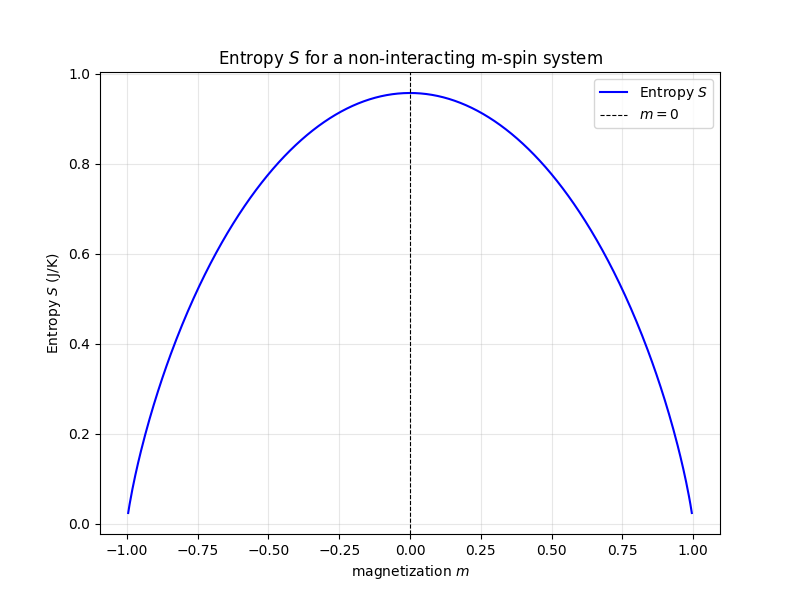
\includegraphics[width=\textwidth]{images/statistical-physics/s-mc-spin-system.png}
        \label{fig:image1}
    \end{minipage}
    \hfill
    \begin{minipage}{0.45\textwidth}
        \centering
        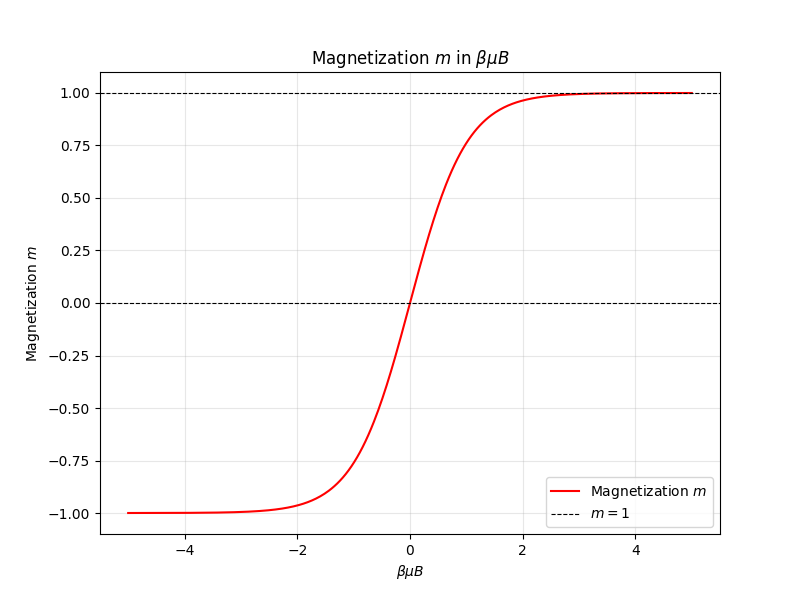
\includegraphics[width=\textwidth]{images/statistical-physics/m-mc-spin-system.png}
        \label{fig:image2}
    \end{minipage}
    \caption{
        Entropy S and magnetization m for a non interacting spin system.
    }
    \label{fig:spin-system}
\end{figure}


\begin{tcolorbox}[colframe=gray!50, colback=gray!10, coltitle=black, title=S and m for a non interacting spin system]

    \begin{equation}
        S=Nk_B\left[\ln{2} -\frac{1}{2}\ln{1-m^2}-\frac{m}{2}\ln{\left(\frac{1+m}{1-m}\right)} \right]
    \end{equation}

    \begin{equation}
        m=\tanh{\left(\beta \mu B\right)}
    \end{equation}

\end{tcolorbox}

\textbf{Proof:}
The multiplicity function of a M magnetized system of N non interacting spins is given by:

\begin{align*}
     & \Omega(N,M)=\frac{N!}{N_{\uparrow}!N_{\downarrow}!}= \frac{N!}{\left( \frac{N+M}{2} \right)!\left( \frac{N-M}{2} \right)!}= \\
     & =\frac{N!}{\left(\frac{N-\frac{U}{\mu B}}{2}\right)! \left(\frac{N+\frac{U}{\mu B}}{2}\right)!}
\end{align*}

The entropy of the system can therefore be calculated:

\begin{align*}
     & S=k_B\ln{\Omega(N,M)}=k_B\ln{\frac{N!}{\left(\frac{N-\frac{U}{\mu B}}{2}\right)! \left(\frac{N+\frac{U}{\mu B}}{2}\right)!}}=...
\end{align*}

Solving the calculation, using the Stirling formula, one finds the aimed form of the entropy.
To find the magnetization, one can derive the entropy in U and find the relation with T, and then revert the relation to find m.

\textbf{Observation}
Regarding S, one can observe that:
\begin{itemize}
    \item $ S \xrightarrow{\underset{m \to 0}{}} k_B \ln{2} $, meaning that the microstates are equiprobable.
    \item $ S \xrightarrow{\underset{m \to 1}{}} 0 $, meaning that the system is in a pure state.
\end{itemize}

Regarding m, one can observe that:
\begin{itemize}
    \item $ m \xrightarrow{\underset{\frac{\mu B}{k_B T} \to 0}{}} 0 $, meaning that the thermal agitation is dominant on the magnetic field.
    \item $ m \xrightarrow{\underset{\frac{\mu B}{k_B T} \to \infty}{}} 1 $, meaning that the magnetic field is dominant on the thermal agitation.
\end{itemize}



\newpage

\begin{tcolorbox}[colframe=gray!90, colback=gray!5, coltitle=white, sharp corners, title=\textbf{Microcanonical Ensamble, Summary}, fonttitle=\large\bfseries]
    \textbf{Gibbs Entropy}
    \vspace{0.5em}

    \begin{equation}
        S_G = -k_B \sum_{i} p_i \ln{p_i}
    \end{equation}
\end{tcolorbox}

\newpage

\section{The Canonical Ensamble}

An ensamble of closed systems in thermal contact with a bath is called Canonical.
This implies that the constrains of this ensamble are N, T and V, meaning that the
energy can instead fluctuate around a mean value U.

\subsection{Canonical Partition Function}

\begin{tcolorbox}[colframe=gray!50, colback=gray!10, coltitle=black, title=Canonical Partition Function]
    \begin{equation}
        Z = \sum e^{-\beta \epsilon_j}
    \end{equation}

    where $\epsilon_j$ is the energy of the j-th microstate.
\end{tcolorbox}

Maximizing the Gibbs entropy similiarly as done for the microcanonical ensamble, but with the constraint of fixed energy, one finds the partition function:

\begin{align*}
     & S= -k_B\sum_{j}p_j\ln{p_j}-\lambda\left(\sum_{j}p_j-1\right)-\beta\left(\sum_{j}\epsilon_jp_j-U\right) \\
     & \frac{dS}{dp_j}=0 \Longrightarrow p_j=e^{-\beta\epsilon_j-\lambda-1} \Longrightarrow                   \\
     & \Longrightarrow 1=e^{-(1+\lambda)}\sum_{j}e^{-\beta\epsilon_j}                                         \\
     & Z\equiv e^{1+\lambda}=\sum_{j}e^{-\beta\epsilon_j} \Longrightarrow p_j=\frac{e^{-\beta\epsilon_j}}{Z}
\end{align*}

As expected, the probability of a microstate is no longer uniform, but depends on its energy.
As a matter of fact, one can find the microcanonical probability if all the microstates have the same energy.

Therefore, the entropy can be rewritten in terms of the partition function Z:

\begin{equation}
    S=k_B\ln{Z}+k_B\beta U
\end{equation}

\subsubsection{$\beta$ Lagrange multiplier}

The physical content of the $\beta$ multiplier can be derived from computing
an infinitesimal variation of the entropy:

\begin{align*}
     & \delta S= S(p_j+\delta p_j)-S(p_j) = -k_B\sum_{j}(\ln{(p_j+\delta p_j)}-\ln{p_j})=...=                                                            \\
     & = -k_B\beta\delta U \Longrightarrow \beta=\frac{1}{k_B}\frac{\delta S}{\delta U}\simeq \frac{1}{k_B}\frac{\partial S}{\partial U}= \frac{1}{k_BT}
\end{align*}

Or, in a quicker way, one can simply differentiate the entropy with respect to the energy:

\begin{equation}
    \beta=\frac{\partial S}{\partial U}= \frac{1}{k_BT}
\end{equation}

\subsection{Free Energy}
From the expression of the entropy, abiding thermodinamical consistance, one can find the Helmholtz free energy F:

\begin{tcolorbox}[colframe=gray!50, colback=gray!10, coltitle=black, title=Helmholtz Free Energy]
    \begin{equation}
        F = U - TS = -k_BT \ln{Z}
    \end{equation}
\end{tcolorbox}

Maximizing the entropy is hence equivalent to minimizing the free energy of Helmotz.

\subsection{Thermodynamical Quantities from Z}

Knowing F, one can derive all the thermodynamical quantities of the system, such as the internal energy U, the entropy S, the pressure P, the Gibbs free energy G and the enthalpy H, in terms of the partition function Z.

\subsubsection{Entropy S}

\begin{align*}
     & S = -\left( \frac{\partial F}{\partial T} \right)_{N,V} = k_B \ln{Z} + k_B T \left( \frac{\partial \ln{Z}}{\partial T} \right)_{N,V}
\end{align*}

\subsubsection{Internal Energy U}

\begin{align*}
     & U= F+TS= -k_B T \ln{Z}-T\left( \frac{\partial F}{\partial T} \right)_{N,V}=                                 \\
     & = -k_B T^2 \left( \frac{\partial \ln{Z}}{\partial T} \right)_{N,V}= -\frac{\partial}{\partial \beta} \ln{Z}
\end{align*}

\subsubsection{Pressure P}

\begin{align*}
    P=-\frac{\partial U}{\partial V}|_{T,N}=-\frac{\partial F}{\partial V}|_{T,N}=k_B T \frac{1}{Z}\frac{\partial Z}{\partial V}
\end{align*}

\newpage
\subsection{Canonical Ensamble, Examples}

\subsubsection{Two levels system}

\begin{figure}[h!]
    \centering
    \begin{minipage}{0.45\textwidth}
        \centering
        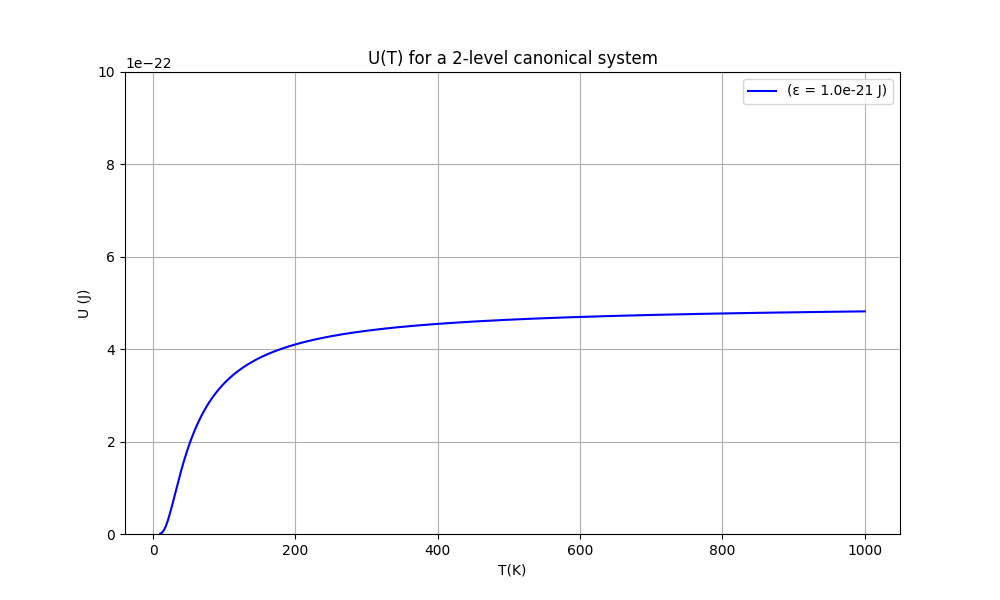
\includegraphics[width=\textwidth]{images/statistical-physics/u-canonical-2-levels.png}
        \label{fig:image1}
    \end{minipage}
    \hfill
    \begin{minipage}{0.45\textwidth}
        \centering
        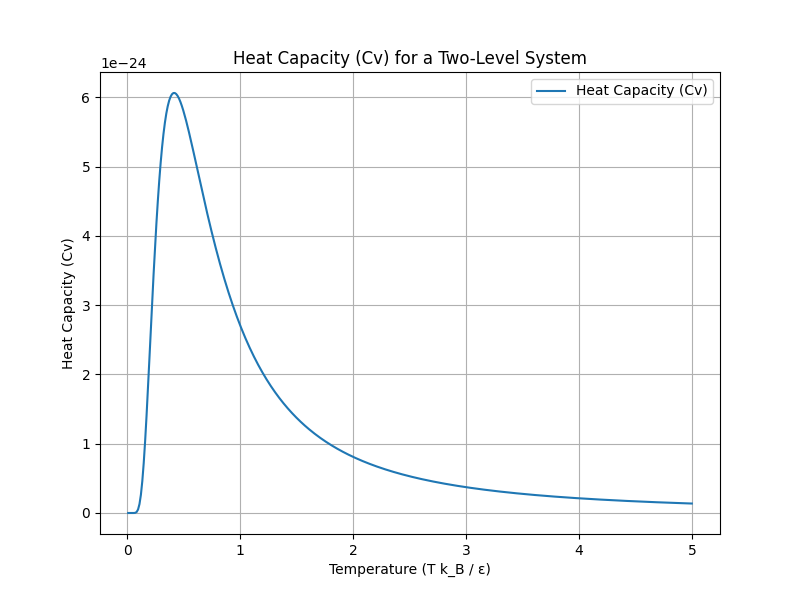
\includegraphics[width=\textwidth]{images/statistical-physics/cv-canonical-2-levels.png}
        \label{fig:image2}
    \end{minipage}
    \caption{
        Internal energy U and heat capacity C$_V$ for a two-level system.
    }
    \label{fig:spin-system}
\end{figure}

Given a system with two energy levels ($\epsilon_0=0$, $\epsilon_1=\epsilon$), the partition function is:

\begin{equation}
    Z=1+e^{-\beta\epsilon}
\end{equation}

The average energy is:

\begin{equation}
    U=-\frac{\partial\ln{Z}}{\partial\beta}= \frac{\epsilon}{1+e^{\beta\epsilon}}
\end{equation}

which is physically consistent, since the energy differences are neglegible at hgh temperatures,
so both energy levels are equally populated. Oppositely, as T goes to zero, the system tends to the ground state.

The heat capacity is given by:

\begin{equation}
    C_V=k_B\left(\frac{\epsilon}{k_BT}\right)^2\frac{e^{\beta\epsilon}}{(1+e^{\beta\epsilon})^2}
\end{equation}

At low temperature, the heat capacity is low, since the only way to increase
U is make the system jump to the second level. Once this happens, the heat capacity increases significantly, reaching the so called Schottky anomaly.
After this, the heat capacity decreases again, since the system is already in the excited state and thermally exciting the system will not affect the energy.


\subsubsection{Quantum simple harmonic oscillator}

\begin{figure}[h!]
    \centering
    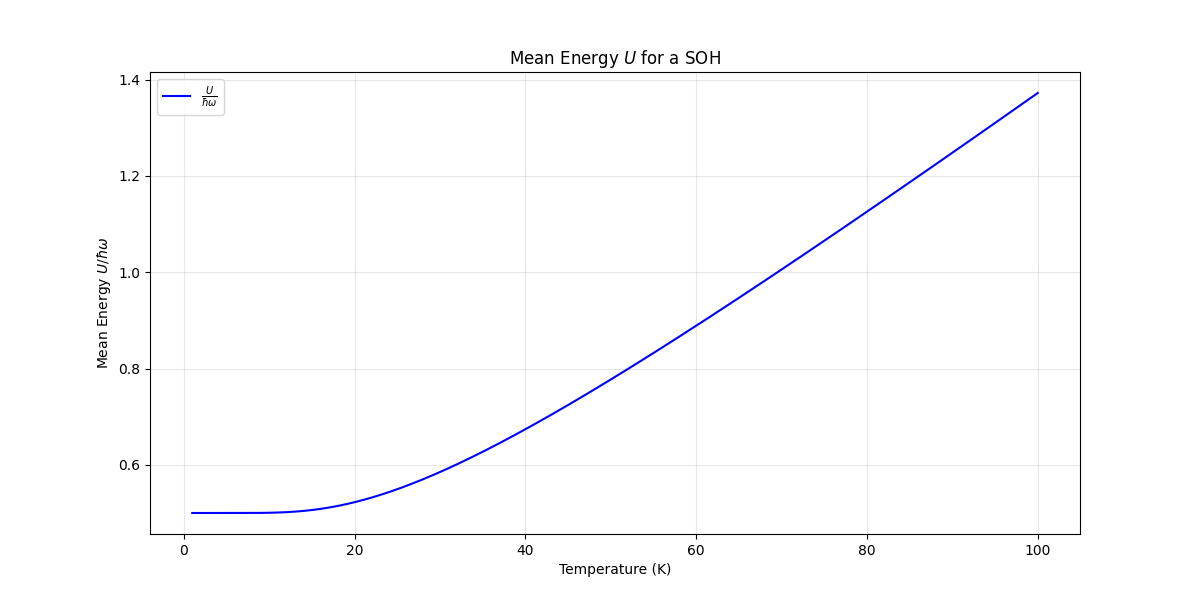
\includegraphics[width=0.5\textwidth]{images/statistical-physics/u-soh.png}
    \caption{
        Internal energy U for a simple harmonic oscillator.
    }
    \label{fig:u-soh}
\end{figure}

Quantizing the simple harmonic oscillator
\footnote{
    The complete quantization of the simple harmonic oscillator can be found in
    \href{https://cesaresabattini.github.io/Physics-Lecture-Notes/}{Quantum Mechanics Notes}.
}
, the energy levels are given by:

\begin{equation}
    \epsilon_n=\hbar\omega\left(n+\frac{1}{2}\right)
\end{equation}

So the partition function is:

\begin{equation}
    Z_Q=\sum e^{-\beta\hbar\omega\left(n+\frac{1}{2}\right)}=\frac{e^{-\frac{\beta\hbar\omega}{2}}}{1-e^{-\beta\hbar\omega}}=\frac{1}{2\sinh{\frac{\beta\hbar\omega}{2}}}
\end{equation}

The average energy is therefore obtainable:

\begin{align*}
    U=-\frac{\partial}{\partial \beta}\ln{Z_Q}=\frac{\hbar \omega}{2}\coth{\frac{\beta\hbar\omega}{2}}
\end{align*}

It's interesting calculating the classical partition function $Z_C$ and show
it to be the limit for high temperatures of the quantum partition function:

\begin{align*}
    Z_C=\int_{-\infty}^\infty\int_{-\infty}^\infty \frac{dp dx}{2\pi \hbar} e^{-\beta\left(\frac{p^2}{2m}+\frac{1}{2}m\omega^2x^2\right)}=\frac{1}{\beta\hbar\omega}
\end{align*}

where the $\frac{1}{2\pi\hbar}$ factor is introduce for consistency with the quantum partition function.
To solve the integral, one can use the gaussian integral formula.

Now one can note $Z_C$ to be the limit of $Z_Q$ for high temperatures:

\begin{align*}
    Z_Q=\frac{e^{-\frac{\beta \hbar \omega}{2}}}{1-e^{-\beta\hbar\omega}}\xrightarrow{{T>>\hbar\omega}}\frac{1}{1-(1-\beta\hbar\omega+ o(\beta\hbar\omega))}=\frac{1}{\beta\hbar\omega}
\end{align*}



\newpage

\begin{tcolorbox}[colframe=gray!90, colback=gray!5, coltitle=white, sharp corners, title=\textbf{Canonical Ensamble, Summary}, fonttitle=\large\bfseries]

    \textbf{Constraints}

    \begin{equation}
        N, T, V
    \end{equation}

    \textbf{Partition Function}

    \begin{equation}
        Z = \sum e^{-\beta \epsilon_j}
    \end{equation}

    \textbf{Helmholtz Free Energy}

    \begin{equation}
        F = U - TS= -k_BT \ln{Z}
    \end{equation}

    \vspace{0.3cm} % Aggiunge uno spazio verticale per separare la sezione precedente dalla tabella
    \textbf{Thermodynamical Quantities from Z}:

    \begin{center}
        \begin{tabular}{|c|c|c|}
            \hline
            \textbf{Name} & \textbf{Definition}                                           & \textbf{Statistical expression}                                           \\ \hline
            \( U \)       & \( U = F + TS \)                                              & \( U = \langle E \rangle = -\frac{\partial}{\partial \beta} \ln Z \)      \\ \hline
            \( S \)       & \( S = -\left( \frac{\partial F}{\partial T} \right)_{N,V} \) & \( S = k_B \ln Z + k_B T \frac{\partial \ln Z}{\partial T} \Big|_{N,V} \) \\ \hline
            \( P \)       & \( P = -\left( \frac{\partial F}{\partial V} \right)_{N,T} \) & from \( F \).                                                             \\ \hline
            \( G \)       & \( G = F + PV \)                                              & \( G = -k_B T \ln Z + PV \)                                               \\ \hline
            \( H \)       & \( H = U + PV \)                                              & from \( U \) and \( P \).                                                 \\ \hline
        \end{tabular}
    \end{center}

\end{tcolorbox}


\newpage

\section{Ideal Gas}

An ideal gas in contact with a fixed temperature external bath is well described by the canonical ensamble,
since the constrains are satisfied.

\subsection{Particle distinguishability}

The distinguishability is the property that in statistical mechanics mainly discerns classical particles from quantistic ones,
beside the bosonic and fermionic nature, whether quantum.
This concept has important repercussions on the partition function of the system.


\subsubsection{Distinguishable particles}

\begin{tcolorbox}[colframe=gray!50, colback=gray!10, coltitle=black, title=Distinguishable Particles Partition Function]
    The partition function of N distinguishable particles is:
    \begin{equation}
        Z=Z_1^N
    \end{equation}
\end{tcolorbox}

\textbf{Proof:}
Given a set of N classical distinguishable particles, the partition function is defined as:

\begin{align*}
    Z= \sum_{i} \frac{N!}{\prod_in_i!}e^{-\beta\sum n_i\epsilon_i}=Z_1^N
\end{align*}

where the sum is over all the possible configurations of particles. In the last equality, the multinomial coefficient is used.

\subsubsection{Indistinguishable particles}

The case of indistinguishable particles is hereby treated in the approximation of single occupation, which is valid for low density systems, where the distance between particles is much greater than the De Broglie wavelength,
which directly implies that the product of the occupation numbers for each configuration is one.
Moreover, since the particles are non indexable, the partition function is reduced to that of distinguishable particles, divided by N!:

\begin{tcolorbox}[colframe=gray!50, colback=gray!10, coltitle=black, title=Indistinguishable Particles Partition Function]
    The partition function of N indistinguishable particles is:
    \begin{equation}
        Z=\frac{Z_1^N}{N!}
    \end{equation}
\end{tcolorbox}
\subsection{Monoatomic quantum ideal gas in a box}

\begin{tcolorbox}[colframe=gray!50, colback=gray!10, coltitle=black, title=Monoatomic Quantum Ideal Gas Z and F]
    The partition function of a quantum ideal gas in a box, in the low density approximation, is:
    \begin{equation}
        Z=\frac{1}{\sqrt{2\pi N}}\left(\frac{g_s e n_Q}{n}\right)^N
    \end{equation}

    where $n_Q$ is the number of quantum concentration and $g_s$ is the spin degeneracy of a particle.
    The Helmotz free energy is:

    \begin{equation}
        F=-Nk_BT\ln{\frac{n_QV}{N}}-Nk_BT
    \end{equation}
\end{tcolorbox}

\textbf{Proof:}
In the model of a gas constrained in an infinite potential well, the single particle partition function is given by
\footnote{
    The complete derivation of the energy for a quantum particle constrained in a box can be found in
    \href{https://cesaresabattini.github.io/Physics-Lecture-Notes/}{Quantum Mechanics Notes}.
}

\begin{align*}
     & Z=\sum e^{-\frac{-\pi^2\hbar^2}{2mL^2}(n_x^2+n_y^2+n_z^2)\beta}=  \\
     & \sum e^{-\frac{\pi^2\hbar^2}{2mL^2k_bT}(n_x^2+n_y^2+n_z^2)}\equiv \\
     & \equiv\sum e^{-\frac{\theta_t}{T}(n_x^2+n_y^2+n_z^2)}=            \\
     & =\left(\sum e^{-\frac{\theta_tn_x^3}{T}}\right)^3
\end{align*}


For $T>>\theta_t$, the sum is approximated by an integral:
\begin{align*}
     & Z \xrightarrow{T>>\theta_t} \left(\int_{0}^{\infty} e^{-\frac{\theta_tn^2}{T}}dn\right)^3=                                                      \\
     & =\left(\frac{1}{2}\sqrt{\frac{\pi T}{\theta_t}}\right)^3= \left(\frac{mk_bT}{2\pi\hbar^2}\right)^{\frac{3}{2}}V= n_QV= \frac{V}{\lambda_{dB}^3}
\end{align*}


where $\lambda_{dB}$ is the De Broglie wavelength of the particle, so $n_Q$ is the number of quantum states density in the semiclassical limit.

\begin{figure}[h]
    \centering
    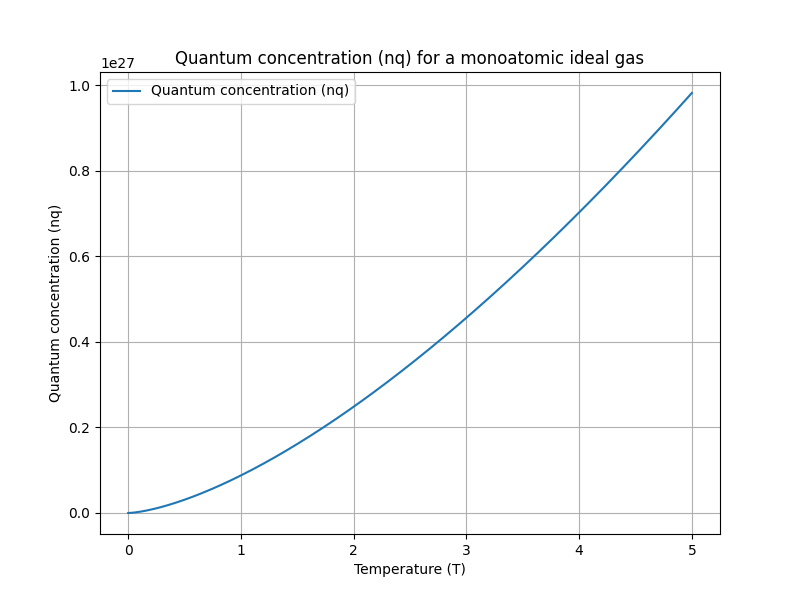
\includegraphics[width=0.5\textwidth]{images/statistical-physics/nq-monoatomic-ideal-gas.png}
    \caption{Quantum state density $n_Q$ as a function of temperature.}
    \label{fig:nq}
\end{figure}

When N particles are considered, the partition function is:

\begin{align*}
    Z=\frac{Z_1^N}{N!}=\frac{(n_QV)^N}{N!}\simeq \frac{1}{\sqrt{2\pi N}}\left(\frac{g_sen_Q}{n}\right)^N
\end{align*}

where $g_s$ is the spin degeneracy of the particle.

Now it's possible to find the expression for the free energy F:

\begin{align*}
    F=-k_BT\ln{Z}=-Nk_BT\ln{\frac{n_QV}{N}}-Nk_BT
\end{align*}

where the term in $ln(2\pi N)$ has been neglected in the limit of large N.


\subsection{Properties of the monoatomic ideal gas}

Any property of the ideal gas can be derived from the partition function,
simply using its definition and the canonical bridge equation, given by the Helmholtz free energy.

\subsubsection{Perfect gas law}

From the expression of F, one can find the pressure of the gas:

\begin{equation}
    P=-\left(\frac{\partial F}{\partial V}\right)_{T,N}=\frac{Nk_BT}{V}
\end{equation}

which can be rearranged to the well known perfect gas law:

\begin{align*}
    PV=nRT
\end{align*}


\subsubsection{Entropy of mixing}

A curious property of the ideal gas is the entropy of mixing, derivable from the partition function Z and
leading to the Sackur-Tetrode equation:

\begin{tcolorbox}[colframe=gray!50, colback=gray!10, coltitle=black, title=Sackur-Tetrode Equation]
    The entropy of an ideal gases is:
    \begin{equation}
        S=-Nk_b\left[\ln{\frac{n_QV}{N}}+\frac{5}{2}\right]
    \end{equation}

\end{tcolorbox}

Here we can distinguish two cases:

\begin{itemize}
    \item Two separated systems, composed by the same type of particle, have a null entropy variation when mixed.


          \begin{align*}
               & S_i=2Nk_b\left[\ln{\frac{n_QV}{N}}+\frac{5}{2}\right]   \\
               & S_f=2Nk_b\left[\ln{\frac{n_Q2V}{2N}}+\frac{5}{2}\right] \\
               & \Delta S=0
          \end{align*}


    \item Two separated systems, composed by two types of particles, have a positive entropy variation when mixed.


          \begin{align*}
               & S_i=Nk_b\left[\ln{\frac{n_Q^AV}{N}}+\frac{5}{2}\right]+Nk_b\left[\ln{\frac{n_Q^BV}{N}}+\frac{5}{2}\right]    \\
               & S_f= Nk_b\left[\ln{\frac{2n_Q^AV}{N}}+\frac{5}{2}\right]+Nk_b\left[\ln{\frac{2n_Q^BV}{N}}+\frac{5}{2}\right] \\
               & \Delta S=2Nk_b\ln{2}
          \end{align*}

\end{itemize}

This is no surprise, since the particles are indistinguishable, so the reversibility of the process is different in the two instances.

\subsection{Quantum ideal diatomic gas in a box}

To derive the partition function for a free diatomic gas, one can follow
an akin procedure to the confined monoatomic case, but considering that the rotational degree implies another energy term:

\begin{equation}
    E_{n,l}=\frac{\hbar^2\pi^2 \textbf{n}^2}{2mL^2}\frac{\hbar^2 l(l+1)}{2I}
\end{equation}

where n is the quantum number of the translational energy, l is the quantum number of the rotational energy and I is the moment of inertia of the molecule.
So, the partition function is given by:

\begin{equation}
    Z=\sum_{\left\{ n,l \right\}} e^{-\beta E_{n,l}}=\sum_{n=0}^\infty e^{-\beta\frac{\hbar^2\pi^2 \textbf{n}^2}{2mL^2}}\sum_{l=0}^{\infty}(2l+1)e^{-\beta\frac{\hbar^2 l(l+1)}{2I}}=Z_nZ_r
\end{equation}

\subsection{Energy equipartition theorem}

\begin{tcolorbox}[colframe=gray!50, colback=gray!10, coltitle=black, title=Energy Equipartition Theorem]

    \begin{equation}
        U=\frac{n}{2}k_BT
    \end{equation}
    where \( n \) is the number of quadratic degrees of freedom of the system.

\end{tcolorbox}

\textbf{Proof:}

\begin{align*}
     & E({x_i})=\sum_{i}^{N}\epsilon_i(x_i)=\sum_{i}^{N}c_ix_i^2                                                                                                 \\
     & U=<E>=<\sum_{i}^{N}\epsilon_i>=\sum_{i}^{N}<\epsilon_i>                                                                                                   \\
     & <\epsilon_j>=\int \prod_{i}^{N}dx_i\epsilon_jP(\epsilon_j)= \frac{\int d\eta \epsilon_je^{-\beta \sum \epsilon_i}}{\int d\eta e^{-\beta \sum \epsilon_i}} \\
     & = \frac{\int dx_j\epsilon_je^{-\beta \epsilon_j}}{\int dx_je^{-\beta \epsilon_j}}=\frac{1}{2}k_bT
\end{align*}

\newpage

\begin{tcolorbox}[colframe=gray!90, colback=gray!5, coltitle=white, sharp corners, title=\textbf{Ideal Gas, Summary}, fonttitle=\large\bfseries]
    \textbf{Partition functions}


    \renewcommand{\arraystretch}{1.5}
    \begin{center}
        \begin{tabular}{|c|c|}
            \hline
            \textbf{Distinguishable} & \textbf{Indistinguishable (semiclassical)} \\ \hline
            \( Z = Z_1^N \)          & \( Z = \frac{Z_1^N}{N!} \)                 \\ \hline
        \end{tabular}

    \end{center}


    \textbf{Quantum monoatomic ideal gas in a box}

    \begin{equation}
        Z_1 = \frac{V}{\lambda_{dB}^3}= \left( \frac{mk_bT}{2\pi\hbar^2} \right)^{\frac{3}{2}}V= n_QV
    \end{equation}

    \begin{equation}
        Z_N = \frac{1}{\sqrt{2\pi N}}\left( \frac{g_s n_Q}{n} \right)^N
    \end{equation}

    \textbf{Entropy of mixing}

    \begin{equation}
        S = -Nk_b\left[ \ln{\frac{n_QV}{N}} + \frac{5}{2} \right]
    \end{equation}

    \textbf{Energy Equipartition Theorem}

    \begin{equation}
        U = \frac{n}{2}k_BT
    \end{equation}

\end{tcolorbox}

\newpage


\section{The Grand Canonical Ensamble}

An ensamble of open system in contact with an external bath is called Grand Canonical,
so the energy and the number of particles can fluctuate around mean values.
Therefore, the constrains are T, V, $\mu$, which is the chemical potential.

\subsection{Chemical Potential}

The concept of chemical potential naturally emerges from the minimization of the free energy
of the system composed by the ensamble and the bath, which is therefore canonical.

One, indeed, finds:

\begin{tcolorbox}[colframe=gray!50, colback=gray!10, coltitle=black, title=Chemical Potential]
    \begin{equation}
        \frac{\partial}{\partial N_R}F_R|_{T,V}=\frac{\partial}{\partial N}F_S|_{T,V}\equiv \mu
    \end{equation}
\end{tcolorbox}


Moreover, expanding the differential of the entropy, one finds:

\begin{equation}
    dU=TdS-PdV+\mu dN
\end{equation}

which is nothing but the most general expression of variation of U in terms of the thermodynamical quantities.

This explicits the physical meaning of the chemical potential: it is the energy required to add a particle to the system,
at constant entropy and volume.

Or, equivalently the free energy required to add a particle to the system at constant temperature and volume.

Or, again, equivalently, the Gibbs energy required to add a particle to the system at constant temperature and pressure.

\subsubsection{Chemical potential for ideal gases}

\begin{figure}[h!]
    \centering
    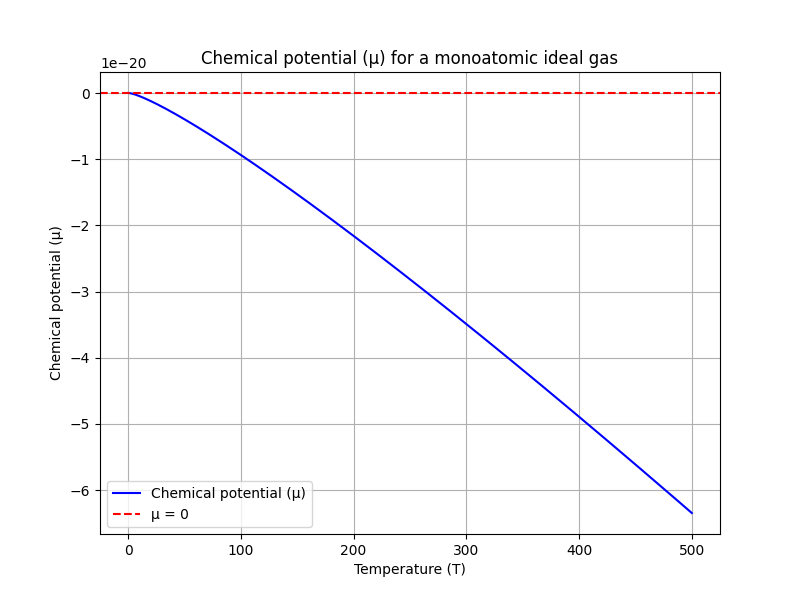
\includegraphics[width=0.5\textwidth]{images/statistical-physics/mu-monoatomic-ideal-gas.png}
    \caption{Chemical potential for a monoatomic ideal gas, as a function of temperature.}
    \label{fig:chemical-potential}
\end{figure}

The chemical potential for a monoatomic ideal gas can be derived from the Free energy F:

\begin{tcolorbox}[colframe=gray!50, colback=gray!10, coltitle=black, title=Chemical Potential for an Ideal Gas]

    \begin{equation}
        \mu=\left( \frac{\partial F}{\partial N} \right)_{T,V}=k_BT\ln{\left( \frac{N}{n_QV} \right)}
    \end{equation}

\end{tcolorbox}

The chemical potential for a diatomic ideal gas is different, since there are 2 additional degrees of freedom (neglecting the vibrational one):

\begin{tcolorbox}[colframe=gray!50, colback=gray!10, coltitle=black, title=Chemical Potential for a
        Diatomic Ideal Gas]

    \begin{equation}
        \mu=k_BT\ln{\left( \frac{n}{n_QZ_r} \right)}
    \end{equation}

    where $Z_r$ is the rotational partition function, which is given by (if $T>>\theta_r$):

    \begin{equation}
        Z_r=\sum_{l=0}^{\infty}(2l+1)e^{-\beta\frac{\hbar^2 l(l+1)}{2I}}\simeq \frac{T}{\theta_r}
    \end{equation}
\end{tcolorbox}

To understand the physical meaning of the trend of $\mu$ for a diatomic gas, one can rewrite it as:

\begin{align*}
    \mu=k_BT\ln{\left( \frac{P}{n_QZ_rk_BT} \right)}
\end{align*}

If the pressure of the gas increases, more energy is required to add a particle, keeping S and V constant.

For high densities, this is no longer valid, since the quantum effects are no longer negligible.

\subsection{Grand Canonical Partition Function}

The process of derivation of the partition function for the grand canonical ensamble is analogous to the canonical one,
meaning it goes through the maximization of the entropy of the system.

One finds:

\begin{tcolorbox}[colframe=gray!50, colback=gray!10, coltitle=black, title=Grand Canonical Partition Function]
    \begin{equation}
        \Xi= \sum_{N=0}^{+\infty}Z(N)e^{\beta\mu N}
    \end{equation}
\end{tcolorbox}

\subsection{Grand Potential}

Thanks to the expression of the grand canonical partition function, the
entropy can be written as:

\begin{align*}
    S= k_bT\ln{\Xi}+\frac{U-\mu N}{T}
\end{align*}

which can be rearranged defining the Grand Potential $\Phi$:

\begin{tcolorbox}[colframe=gray!50, colback=gray!10, coltitle=black, title=Grand Potential]
    \begin{equation}
        \Phi=k_bT\ln{\Xi}=\mu N-F
    \end{equation}
\end{tcolorbox}

from which any thermodinamical quantity is obtainable, as shown in the compendium.

For example, the average number of particle is:

\begin{equation}
    \mathcal{N}=<N>=\frac{\sum_{N=0}^{+\infty} N Z(N)e^{\mu N}}{\Xi}= \frac{\partial}{\partial \mu}\Phi
\end{equation}

\newpage

\subsection{Grand Canonical Ensamble, Excercises}

\begin{tcolorbox}[colframe=orange!60, colback=gray!5, coltitle=black, title=\textbf{Kennett, 6.4}, fonttitle=\large\bfseries]

    Consider a two-level system with energy levels 0 and $\epsilon$ populated by bosons (bosons
    have norestrictions on how many particles can be in each energy level). Find the
    average energy and occupation of the levels and calculate the heat capacity.

\end{tcolorbox}

\textbf{Solution:}

To find the Grand Canonical partition function $\Xi$, one surely cannot use the semiclassical approximation
of dilute gas; so there's not an immediate formulae to use.
Therefore, one can proceed in the following way: study the partition function
summing on the couples $(n_0, n_1)$, occupation numbers of the two levels, with the constrain
of the total number of particles N, and then take the limit of the infinite number of particles:

\begin{equation}
    \begin{aligned}
         & \Xi=\sum_{N=0}^{\infty}\sum_{j}Z(N)e^{\beta\mu N}=\sum_{\left\{ (n_1,n_2) \right\}} e^{-\beta(n_1\epsilon_1+n_2\epsilon_2)}e^{\beta\mu(n_1+n_2)}=                                     \\
         & =\sum_{n_1=0}^{N}e^{-\beta n_1\epsilon_1}e^{\beta\mu n_1}\sum_{n_2=0}^{N-n_1}e^{-\beta n_2\epsilon_2}e^{\beta\mu n_2}=                                                                \\
         & =\sum_{n_1=0}^{N}e^{-\beta n_1 (\epsilon_1-\mu)}\frac{1-e^{-\beta(\mu-\epsilon_2)(N+1)}}{1-e^{-\beta(\mu-\epsilon_2)}}=                                                               \\
         & =\frac{1-e^{-\beta(\mu-\epsilon_2)(N+1)}}{1-e^{-\beta(\mu-\epsilon_2)}}\sum_{n_1=0}^{N}e^{-\beta n_1 (\epsilon_1-\mu)}=                                                               \\
         & =\frac{1-e^{-\beta(\mu-\epsilon_2)(N+1)}}{1-e^{-\beta(\mu-\epsilon_2)}}\frac{1-e^{-\beta(\epsilon_1-\mu)(N+1)}}{1-e^{-\beta(\epsilon_1-\mu)}}\Longrightarrow_{N\Longrightarrow\infty} \\
         & \Longrightarrow_{N\Longrightarrow\infty}=\frac{1}{1-e^{-\beta(\mu-\epsilon_2)}}\frac{1}{1-e^{-\beta(\epsilon_1-\mu)}}= \frac{1}{1-e^{-\beta(\mu-\epsilon)}}\frac{1}{1-e^{\beta\mu}}
    \end{aligned}
\end{equation}

Now that $\Xi$ is found, one can find the average occupation of the levels from the great potential $\Phi$:

\begin{equation}
    \begin{aligned}
         & \mathcal{N}= \frac{\partial \Phi}{\partial \mu}= \frac{\partial}{\partial \mu}\left(k_B T \ln{\Xi}\right)= \\
         & \sum_{j=0}^{1}\frac{1}{1-e^{\beta(\epsilon_j-\mu)}}= \sum_{j=0}^{1} <n_j>
    \end{aligned}
\end{equation}

The average energy U is defined as:

\begin{equation}
    \begin{aligned}
         & U=\sum_{j=0}^{1} <n_j>\epsilon_j= \frac{\epsilon_0}{1-e^{\beta(\epsilon_0-\mu)}}+\frac{\epsilon_1}{1-e^{\beta(\epsilon_1-\mu)}}= \\
         & =\frac{\epsilon}{e^{\beta(\epsilon-\mu)}-1}
    \end{aligned}
\end{equation}

The heat capacity is hence given by:

\begin{equation}
    \begin{aligned}
         & C_V=\frac{\partial U}{\partial T}= \frac{\partial U}{\partial \beta}\frac{\partial \beta}{\partial T}= \frac{\partial U}{\partial \beta}\frac{1}{k_B T^2}= \\
         & =\frac{\epsilon (\epsilon-\mu)}{k_B T^2}\frac{e^{\beta(\epsilon-\mu)}}{(e^{\beta(\epsilon-\mu)}-1)^2}
    \end{aligned}
\end{equation}



\newpage
\begin{tcolorbox}[colframe=gray!90, colback=gray!5, coltitle=white, sharp corners, title=\textbf{Grand Canonical Ensamble, Summary}, fonttitle=\large\bfseries]

    \textbf{Constraints}

    \begin{equation}
        T, V, \mu
    \end{equation}

    \textbf{Chemical Potential}

    \begin{equation}
        \mu = \left( \frac{\partial F}{\partial N} \right)_{T,V}
    \end{equation}

    \textbf{Grand Canonical Partition Function}

    \begin{equation}
        \Xi = \sum_{N=0}^{+\infty} Z(N)e^{\beta\mu N}
    \end{equation}

    \textbf{Grand Potential}

    \begin{equation}
        \Phi = k_bT\ln{\Xi} = \mu N - F
    \end{equation}

    \textbf{\(\mu \) for an ideal gas}

    \begin{equation}
        \mu=
        \left\{
        \begin{aligned}
             & k_BT\ln{\left( \frac{N}{n_QV} \right)} \quad , \quad \text{if monoatomic}  \\
             & k_BT\ln{\left( \frac{n}{n_Q Z_r} \right)} \quad , \quad \text{if diatomic}
        \end{aligned}
        \right.
    \end{equation}

    \vspace{0.3cm}
    \textbf{Thermodynamical Quantities from \(\Phi \)}

    \begin{center}
        \begin{tabular}{|c|c|}
            \hline
            \textbf{Name}     & \textbf{Statistical Expression}                                \\ \hline
            \( \mathcal{N} \) & \( -\left( \frac{\partial \Phi}{\partial \mu} \right)_{T,V} \) \\ \hline
            \( S \)           & \( -\left( \frac{\partial \Phi}{\partial T} \right)_{V,\mu} \) \\ \hline
            \( P \)           & \( -\left( \frac{\partial \Phi}{\partial V} \right)_{T,\mu} \) \\ \hline
            \( G \)           & \( \Phi + PV \)                                                \\ \hline
        \end{tabular}
    \end{center}

\end{tcolorbox}

\newpage

\section{Quantum Statistical Mechanics}

\begin{figure}[h]
    \centering
    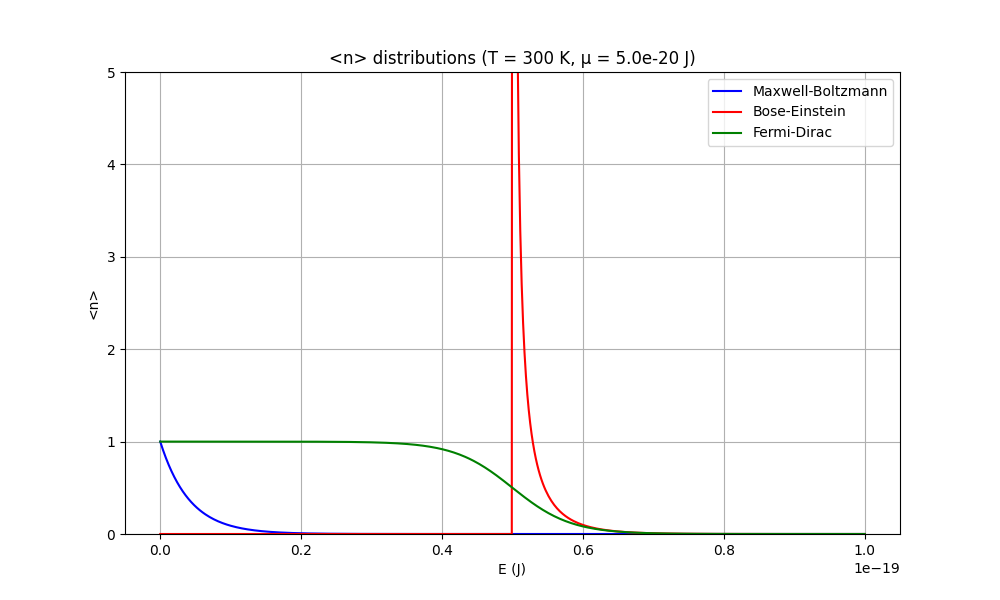
\includegraphics[width=0.5\textwidth]{images/statistical-physics/n-distributions.png}
    \caption{Quantum statistics for different types of particles.}
    \label{fig:quantum-statistics}
\end{figure}

\subsection{Maxwell Boltzmann Statistics}

The Maxwell-Boltzmann statistics describes an ensable of non interacting quantum particles in the classical
approximation of dilute gas, meaning the grand canonical partition function is:

\begin{equation}
    \Xi=\sum_{N=0}^{+\infty}\frac{Z^N}{N!}e^{\beta\mu N}
\end{equation}

Therefore, the average number of particles per energy level is obtainable from the great potential as:

\begin{equation}
    \mathcal{N}=\frac{1}{\beta}\frac{\partial}{\partial \mu}\ln{\Xi}=\sum_{s} e^{-\beta(\epsilon_s-\mu)}
\end{equation}

so that:

\begin{equation}
    <n_s>=e^\beta(\mu-\epsilon_s)
\end{equation}


\subsection{Fermi-Dirac Statistics}

The Fermi-Dirac statistics is necessary whenever the fermionic nature of the particles
can't be disregarded.
It can be derived from the grand canonical partition function, and it is given by:

\begin{equation}
    <n_s>=\frac{1}{e^{\beta(\epsilon_s-\mu)}+1}
\end{equation}

Some physical observations are suitable:

\begin{itemize}
    \item The average number of particles per energy level is always less than 1.
    \item If $\mu>\epsilon_s$, as T goes to 0, the average number of particles per energy level goes to 1,
          whereas if $\mu<\epsilon_s$, it goes to 0. This implies that the average number of particles per energy level tends to
          the Heaviside step function.
    \item The T=0 potential is called Fermi Energy, and it is the energy of the highest occupied state.
\end{itemize}

\subsection{Bose-Einstein Statistics}

The Bose-Einstein statistics is necessary whenever the bosonic nature of the particles
can't be disregarded.
It can be derived from the grand canonical partition function, and it is given by:

\begin{equation}
    <n_s>=\frac{1}{e^{\beta(\epsilon_s-\mu)}-1}
\end{equation}

Some physical observations are suitable:

\begin{itemize}
    \item The average number of particles per energy level is always greater than 1.
    \item If $\mu<\epsilon_s$, as T goes to 0, the average number of particles per energy level goes to 0,
          whereas if $\mu>\epsilon_s$, it goes to -1, which is non-physical. This behaviour is indeed prevented by
          the fact that the chemical potential is never greater than the energy of the state, at any temperature.
\end{itemize}


\subsection{Density of States}

\begin{figure}[h]
    \centering
    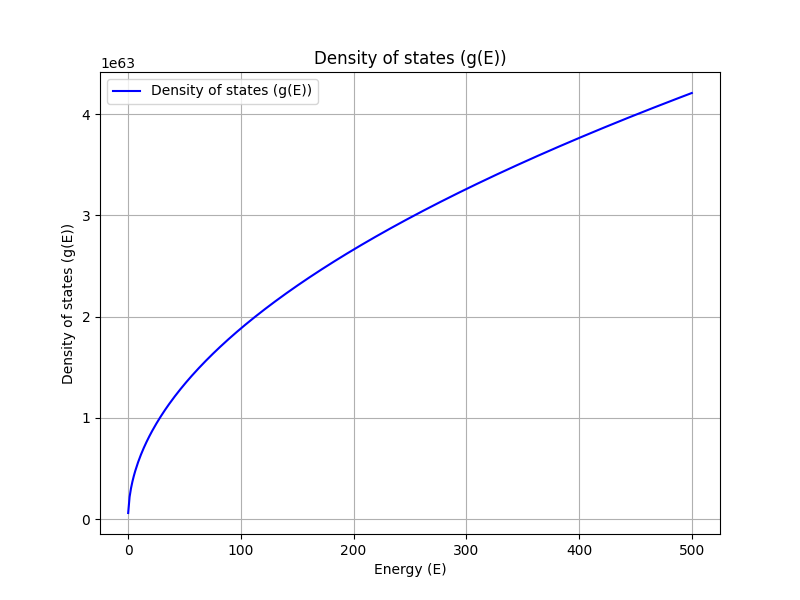
\includegraphics[width=0.5\textwidth]{images/statistical-physics/state-density.png}
    \caption{Density of states as a function of energy.}
    \label{fig:density-of-states}
\end{figure}

\begin{tcolorbox}[colframe=gray!50, colback=gray!10, coltitle=black, title=Number of states]
    The number of states in the limit of a continuus spectrum is given by:

    \begin{equation}
        N=\int \frac{g_s}{4\pi^2}\left( \frac{2m}{\hbar^2} \right)^{\frac{3}{2}}V\sqrt{\epsilon} <n>d\epsilon
    \end{equation}
\end{tcolorbox}

\textbf{Proof:}
The energy for a gas confined in a 3D box is given by:

\begin{equation}
    \epsilon=\frac{\pi^2\hbar^2}{2m}(n_x^2+n_y^2+n_z^2)
\end{equation}

In the limit of a continuus spectrum, the number of states for $E<\epsilon$ is given by the volume of the
positive octant of the sphere in the 3D space of the wave numbers:

\begin{equation}
    N(E<\epsilon)= \frac{1}{8} \frac{4}{3}\pi \left(\sqrt{\frac{V^\frac{2}{3} \epsilon 2m}{\hbar^2\pi^2}}\right)^3
\end{equation}

Therefore, one can directly find the density of states:

\begin{equation}
    dN\simeq\frac{dN}{dE}dE=\frac{1}{4\pi^2}\left(\frac{2m}{\hbar^2}\right)^{\frac{3}{2}}V\sqrt{\epsilon}d\epsilon=g(\epsilon)d\epsilon
\end{equation}

\newpage
\begin{tcolorbox}[colframe=gray!90, colback=gray!5, coltitle=white, sharp corners, title=\textbf{Quantum Statistical Mechanics, Summary}, fonttitle=\large\bfseries]
    \textbf{Maxwell-Boltzmann Statistics}

    \begin{equation}
        <n_s>=e^{\beta(\mu-\epsilon_s)}
    \end{equation}

    \textbf{Fermi-Dirac Statistics}

    \begin{equation}
        <n_s>=\frac{1}{e^{\beta(\epsilon_s-\mu)}+1}
    \end{equation}

    \textbf{Bose-Einstein Statistics}

    \begin{equation}
        <n_s>=\frac{1}{e^{\beta(\epsilon_s-\mu)}-1}
    \end{equation}

    \textbf{3D Density of States}

    \begin{equation}
        g(\epsilon)=\frac{g_s}{4\pi^2}\left( \frac{2m}{\hbar^2} \right)^{\frac{3}{2}}V\sqrt{\epsilon}
    \end{equation}

    \textbf{Thermal Average}

    \begin{equation}
        <y(E)>=\frac{1}{N}\sum_{s}y(\epsilon_s)<n_s>\Longrightarrow \frac{1}{N}\int_0^{+\infty}g(\epsilon)y(\epsilon)f(\epsilon)d\epsilon
    \end{equation}
\end{tcolorbox}
\newpage

\section{Fermions}

Hereby it's presented the derivation of the chemical potential for a Fermi gas,
fist for T=0 and then for T>0, in the Sommerfeld approximation.

\subsection{Fermi Gas at T=0}

\begin{figure}[h]
    \centering
    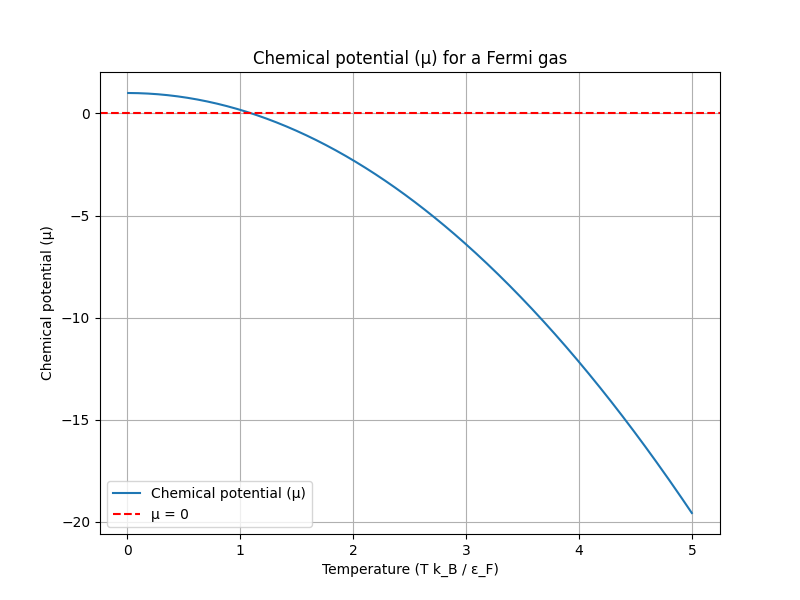
\includegraphics[width=0.5\textwidth]{images/statistical-physics/mu-fermions.png}
    \caption{Chemical potential as a function of temperature for a Fermi gas.}
    \label{fig:mu-fermions}
\end{figure}

First of all, the Fermi-Dirac distribution is:

\begin{equation}
    <n_s>=\frac{1}{e^{\beta(\epsilon_s-\mu)}+1}
\end{equation}

At T=0, it can be approximated with the Heaviside step function:

\begin{equation}
    <n_s>=\theta(\mu-\epsilon_s)=
    \left\{
    \begin{aligned}
         & 1 \quad , \quad \epsilon_s<\mu \\
         & 0 \quad , \quad \epsilon_s>\mu
    \end{aligned}
    \right.
\end{equation}

Using the termal average for the number of particle, one finds:

\begin{equation}
    \begin{aligned}
         & \mathcal{N}=\frac{\partial\Psi}{\partial \mu}=\sum_s <n>_s\Longrightarrow^{n\Longrightarrow\infty} \int_{0}^{\infty} d\epsilon g(\epsilon)f(\epsilon)= \\
         & =\int_{0}^{\mu} d\epsilon g(\epsilon)=\frac{g_sV}{4\pi^2}\left(\frac{2m}{\hbar^2}\right)^{\frac{3}{2}}\int_{0}^{\mu}\sqrt{\epsilon}d\epsilon=          \\
         & = \frac{g_sV}{6\pi^2}\left(\frac{2m\mu}{\hbar^2}\right)^{\frac{3}{2}}\Longrightarrow                                                                   \\                                                 \\
         & \Longrightarrow \mu(T=0)=\frac{\hbar^2}{2m}\left(\frac{6\pi^2n}{g_s}\right)^{\frac{2}{3}}\equiv \epsilon_f
    \end{aligned}
\end{equation}

Any other thermodinamic quantity can be now derived, such as the average energy U:

\begin{equation}
    U=\int_{0}^{\mu}d\epsilon g(\epsilon)\epsilon=\frac{3}{5}\epsilon_f\mathcal{N}
\end{equation}

which is actually an important result, stating that the average energy of a Fermi gas at T=0 is 3/5 of the Fermi energy, instead
of 0, as one might expect from a classical interpretation. Indeed, a null energy for a Fermi gas
would violate the Pauli exclusion principle.

It's now possible to define the Fermi temperature:

\begin{equation}
    T_f=\frac{\epsilon_f}{k_b}
\end{equation}

and observe that:

\begin{itemize}
    \item If T=0, $f(\epsilon)=\theta(\mu-\epsilon)$.
    \item If $T<<T_F$, $f(\epsilon)$ is smooth around $\mu$.
    \item If $T>T_F$, $f(\epsilon)$ tends to the Maxwell-Boltzmann distribution.
\end{itemize}

\subsection{Fermi Gas at $T>0$}
\subsubsection{Sommerfeld Expansion}

Sommerfeld perturbative approach is valid for $T<<T_F$, and will be useful to compute $\mu(T>0)$.

\begin{tcolorbox}[colframe=gray!50, colback=gray!10, coltitle=black, title=Sommerfeld expansion]

    \begin{equation}
        I=\int_{0}^{\infty}K(\epsilon)f(\epsilon)d\epsilon \simeq \int_0^\mu d\epsilon K(\epsilon)+\frac{\pi^2}{6}(k_BT)^2K'(\mu)
    \end{equation}

\end{tcolorbox}

\textbf{Proof:}

Given $G(\epsilon)$, $K(\epsilon)$ generic primitive:
\begin{equation}
    \begin{aligned}
         & I=\int_0^\infty K(\epsilon)\frac{1}{e^\beta(\epsilon-\mu)}d\epsilon= \quad \text{partial integration}   \\
         & =f_0(\infty)G(\infty)-f_0(0)G(0)-\int_0^\infty f_0'(\epsilon)G(\epsilon)d\epsilon\simeq                 \\
         & -G(0)+\int_0^\infty G(\epsilon)\left(-\frac{\partial f_0(\epsilon)}{\partial \epsilon} \right)d\epsilon
    \end{aligned}
\end{equation}

Since the derivative of Heaviside step function is the Dirac delta function, and we're working in the limit $T<<T_F$,
one can now expand $G(\epsilon)$ around $\mu$:

\begin{equation}
    \begin{aligned}
         & I\simeq -G(0)+G(\mu)\int_0^\infty d\epsilon\left( -\frac{\partial f_0}{\partial \epsilon} \right) +G'(\mu)\int_0^\infty d\epsilon(\epsilon-\mu)\left( -\frac{\partial f_0}{\partial \epsilon} \right) + \\
         & + \frac{1}{2}G''(\mu)\int_0^\infty d\epsilon(\epsilon-\mu)^2\left( -\frac{\partial f_0}{\partial \epsilon} \right)
    \end{aligned}
\end{equation}

The generic therm multipied by $G^r(\mu)$, can be handled as follows:

\begin{equation}
    \begin{aligned}
         & \frac{1}{r!}\int_0^\infty d\epsilon(\epsilon-\mu)^r\left( -\frac{\partial f_0}{\partial \epsilon} \right)=                                                                      \\
         & = \frac{1}{r!}\int_0^\infty d\epsilon (\epsilon-\mu)^r\frac{\beta e^{\beta(\epsilon-\mu)}}{(e^{\beta(\epsilon-\mu)}+1)^2}= \quad \text{change variable $x=\beta(\epsilon-\mu)$} \\
         & = \frac{(k_BT)^r}{r!}\int_{-\beta\mu}^\infty dx x^r\frac{e^x}{(e^x+1)^2}\simeq \frac{(k_BT)^r}{r!}\int_{-\infty}^\infty dx x^r\frac{e^x}{(e^x+1)^2}
    \end{aligned}
\end{equation}

so we notice that the odd terms vanish, and the even terms are proportional to $(k_BT)^r$.
So:

\begin{equation}
    \begin{aligned}
         & I\simeq -G(0)+G(\mu)+\frac{1}{2}G''(\mu)\int_o^\infty \simeq                                                                                 \\
         & -G(0)+G(\mu)+(k_BT)^2G''(\mu)\int_0^\infty dx \frac{x^2}{(1+e^x)(1+e^{-x})}=                                                                 \\
         & =-G(0)+G(\mu)-(k_BT)2G''(\mu)\frac{\partial}{\partial \alpha}\left[\int_0^\infty dx \frac{xe^{-\alpha x}}{1+e^{-\alpha x}}\right]_{\alpha=1}
    \end{aligned}
\end{equation}

The last integral can be handled this way:

\begin{equation}
    \begin{aligned}
         & -\frac{\partial}{\partial \alpha}\left[\int_0^\infty dx \frac{xe^{-\alpha x}}{1+e^{-\alpha x}}\right]_{\alpha=1}=                               \\
         & =-\sum_{n=0}^ \infty (-1)^n\frac{\partial}{\partial \alpha}\left[ \int_0^\infty dx x e^{-\alpha(n+1)x} \right]_{\alpha=1}=                      \\
         & =-\sum_{n=0}^\infty \frac{(-1)^n}{(n+1)^2}\frac{\partial}{\partial \alpha}\left[\frac{1}{\alpha^2} \right]_{\alpha=1}\int_0^\infty dy y e^{-y}= \\
         & = 2\Gamma(2)\sum_{n=0}^\infty \frac{(-1)^n}{(n+1)^2}=2\sum_{n=0}^\infty \frac{(-1)^n}{(n+1)^2}=\zeta(2)=\frac{\pi^2}{6}
    \end{aligned}
\end{equation}

which leads to:

\begin{equation}
    I\simeq -G(0)+G(\mu)+\frac{\pi^2}{6}(k_BT)^2G''(\mu)
\end{equation}

and, in terms of $K(\epsilon)$:

\begin{equation}
    I=\int_0^\mu d\epsilon K(\epsilon)+\frac{\pi^2}{6}(k_BT)^2K'(\mu)+O(T^4)
\end{equation}

\subsubsection{$\mu(T>0)$}

Substituting the density of states in the Sommerfeld expansion, one finds:

\begin{equation}
    \begin{aligned}
         & \mathcal{N}\simeq \frac{g_sV}{4\pi^2}\left(\frac{2m}{\hbar^2}\right)^{\frac{3}{2}}\left[\int_0^\mu d\epsilon \sqrt{\epsilon}+\frac{\pi^2}{6}(k_BT)^2\frac{1}{2\sqrt{\mu}}\right]= \\
         & =\frac{g_s V}{4\pi^2}\left(\frac{2m}{\hbar^2}\right)\left[\frac{2}{3}\mu^{\frac{3}{2}}+\frac{\pi^2}{6}(k_BT)^2\frac{1}{2\sqrt{\mu}}\right]
    \end{aligned}
\end{equation}

Reverting the equation, one finds, after some algebra:

\begin{tcolorbox}[colframe=gray!50, colback=gray!10, coltitle=black, title= $\mu(T>0)$]

    \begin{equation}
        \begin{aligned}
            \mu(T)\simeq \epsilon_f\left[1-\frac{\pi^2}{12}\left(\frac{k_BT}{\epsilon_f}\right)^2\right]
        \end{aligned}
    \end{equation}
\end{tcolorbox}


\begin{figure}[h]
    \centering
    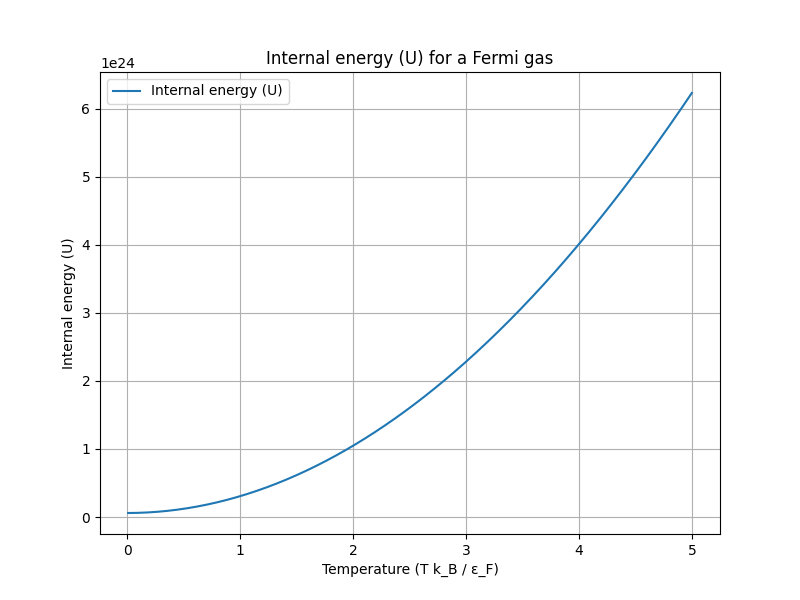
\includegraphics[width=0.5\textwidth]{images/statistical-physics/u-fermions.png}
    \caption{Average energy as a function of temperature for a Fermi gas.}
    \label{fig:u-fermions}
\end{figure}

Using this expression in the Sommerfeld expansion, it's possible to derive the average energy U:

\begin{tcolorbox}[colframe=gray!50, colback=gray!10, coltitle=black, title= $U(T>0)$]

    \begin{equation}
        \begin{aligned}
            U(T)\simeq \frac{3}{5}\epsilon_f\mathcal{N}\left[1+\frac{5\pi^2}{12}\left(\frac{k_BT}{\epsilon_f}\right)^2\right]
        \end{aligned}
    \end{equation}

\end{tcolorbox}

\begin{figure}[h]
    \centering
    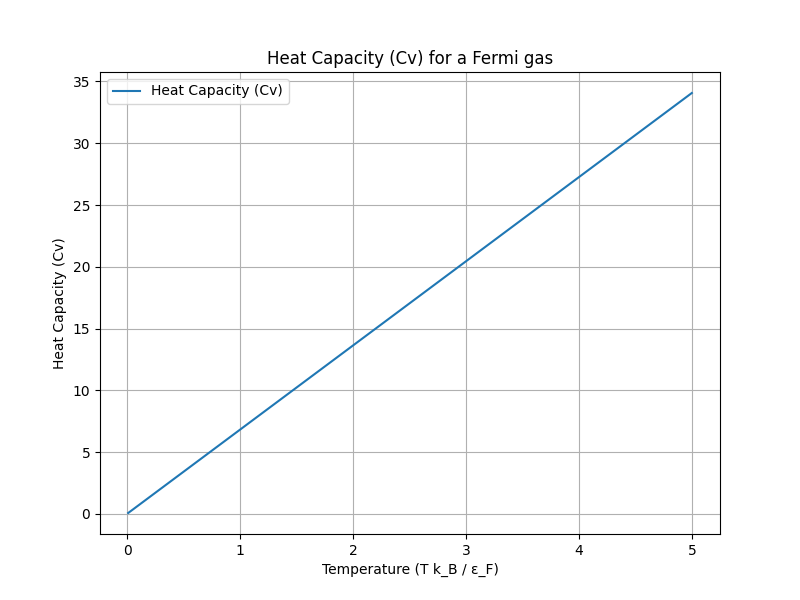
\includegraphics[width=0.5\textwidth]{images/statistical-physics/cv-fermions.png}
    \caption{Heat capacity as a function of temperature for a Fermi gas.}
    \label{fig:fermions-heat-capacity}
\end{figure}
From the average energy, one can derive the heat capacity:

\begin{tcolorbox}[colframe=gray!50, colback=gray!10, coltitle=black, title=$C_V(T>0)$]
    \begin{equation}
        \begin{aligned}
            C_V(T)\simeq \frac{\pi^2}{2}\frac{k_B^2T}{\epsilon_f}N(T)
        \end{aligned}
    \end{equation}
\end{tcolorbox}

\newpage

\newpage
\begin{tcolorbox}[colframe=gray!90, colback=gray!5, coltitle=white, sharp corners, title=\textbf{Fermions, Summary}, fonttitle=\large\bfseries]
    \textbf{Chemical Potential at T=0}

    \begin{equation}
        \mu(T=0)=\epsilon_f=\frac{\hbar^2}{2m}\left(\frac{6\pi^2n}{g_s}\right)^{\frac{2}{3}}
    \end{equation}

    \textbf{Fermi Temperature}

    \begin{equation}
        T_f=\frac{\epsilon_f}{k_b}
    \end{equation}

    \textbf{Chemical Potential at $T>0$}

    \begin{equation}
        \mu(T)\simeq \epsilon_f\left[1-\frac{\pi^2}{12}\left(\frac{k_BT}{\epsilon_f}\right)^2\right]
    \end{equation}

    \textbf{Average Energy at $T>0$}

    \begin{equation}
        U(T)\simeq \frac{3}{5}\epsilon_f\mathcal{N}\left[1+\frac{5\pi^2}{12}\left(\frac{k_BT}{\epsilon_f}\right)^2\right]
    \end{equation}


\end{tcolorbox}
\newpage

\section{Bosons}

Hereby is presented the Bose gas and its peculiar proprties are derived:
the black body radiation and the Bose-Einstein condensation.
But first, let's recall the Bose-Einstein distribution:

\begin{equation}
    <n_s>=\frac{1}{e^{\beta(\epsilon_s-\mu)}-1}
\end{equation}


\subsection{Black body radiation}

\begin{figure}[h]
    \centering
    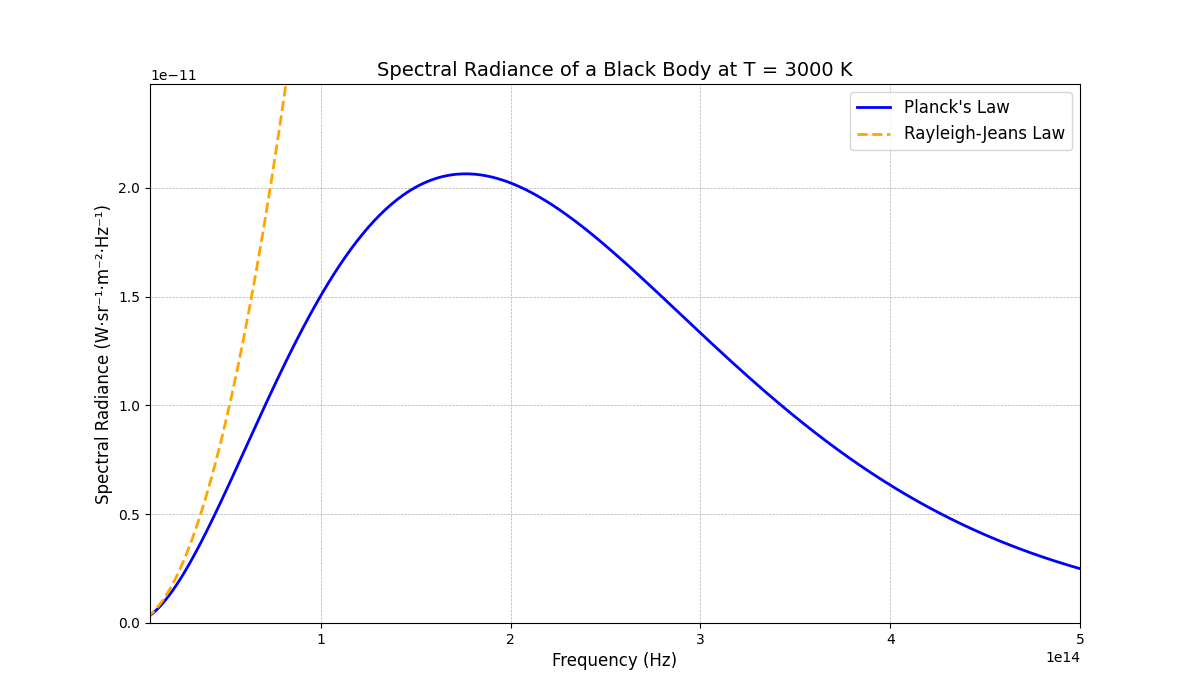
\includegraphics[width=0.5\textwidth]{images/statistical-physics/black-body.png}
    \caption{Black body radiation as a function of frequency.}
    \label{fig:black-body-radiation}
\end{figure}
The density of states for a photon gas in a box is:

\begin{equation}
    g(\omega)=\frac{d N}{d\omega}=\frac{V\omega^2}{\pi^2c^3}
\end{equation}

from which one can calculate the thermal average of the density of photons:

\begin{equation}
    \begin{aligned}
         & \frac{N}{V}\equiv<n>=\frac{1}{V}\int_0^\infty d\omega <n>_\omega g(\omega)=\frac{1}{V}\int_0^\infty d\omega \frac{V\omega^2}{\pi^2c^3}\frac{1}{e^{\beta\hbar\omega}-1}= \\
         & =\frac{1}{\pi^2}\left(\frac{k_B T}{\hbar c}\right)^3\int_0^\infty dx \frac{x^2}{e^x-1}=                                                                                 \\
         & = \frac{1}{\pi^2}\left(\frac{k_B T}{\hbar c}\right)^3 \Gamma(3)\Psi(3)\simeq                                                                                            \\
         & \simeq \frac{2.404}{\pi^2}\left(\frac{k_B T}{\hbar c}\right)^3
    \end{aligned}
\end{equation}

And now one can calculate the energy density, obtaining Planck's law:

\begin{equation}
    V u(\omega)d\omega=\hbar \omega N(\omega)d\omega=\frac{\hbar \omega^3}{\pi^2c^3}\frac{1}{e^{\beta\hbar\omega}-1}V
\end{equation}

which at low frequencies tends to Reyleigh-Jeans law, but prevents the ultraviolet catastrophe:

\begin{equation}
    u_{RJ}(\omega)=\frac{ \omega^2}{\pi^2c^3}k_BT
\end{equation}


\subsection{Bose-Einstein Condensation}

\begin{figure}[h]
    \centering
    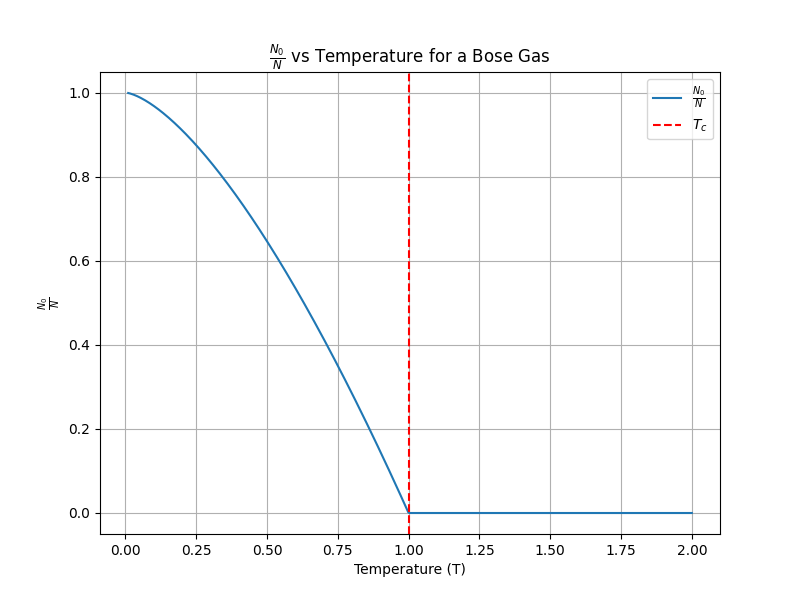
\includegraphics[width=0.5\textwidth]{images/statistical-physics/bose-einstein-condensation.png}
    \caption{Bose-Einstein condensation as a function of temperature.}
    \label{fig:bose-einstein-condensation}
\end{figure}

The Bose Einstein condensation is a phase transition occurring in a Bose gas at low temperatures,
when the number of particles is fixed.

\begin{equation}
    \begin{aligned}
         & N=\int_0^\infty d\epsilon g(\epsilon)\frac{1}{e^{\beta(\epsilon-\mu)}-1}\simeq                                                                                                                                  \\
         & \simeq \int_0^\infty d\epsilon g(\epsilon)\frac{1}{e^{\beta \epsilon}-1}=\frac{g_sV}{4\pi^2}\left(\frac{2m}{\hbar^2}\right)^{\frac{3}{2}}\int_0^\infty d\epsilon \frac{\sqrt{\epsilon}}{e^{\beta_0\epsilon}-1}= \\
         & =g_sV\left(\frac{mk_BT_0}{2\pi\hbar^2}\right)^{\frac{3}{2}}\zeta\left(\frac{3}{2}\right)\simeq 2.612 g_s n_Q(T=0) V= \frac{2.612 g_s}{\lambda_{dB}^3}V
    \end{aligned}
\end{equation}

where $\lambda_{dB}$ is the De Broglie wavelength at T=0.

When such a critical density is reached, the approximation utilized to find $g(\epsilon)$ is no
longer valid, since it would imply $g(0)=0$, which is not what physically happens: the lowest state keeps
absorbing bosons, resulting in the Bose-Einstein condensation.

So the density of states must be corrected, including the ground state:

\begin{equation}
    \begin{aligned}
         & N=<N_0>+g_s V \left(\frac{mk_BT}{2\pi \hbar^2}\right)^{\frac{3}{2}}\zeta\left(\frac{3}{2}\right) \Longrightarrow \\
         & \Longrightarrow \frac{<N_0>}{N}=1-\left(\frac{T}{T_0}\right)^{\frac{3}{2}}
    \end{aligned}
\end{equation}

\subsection{Average Energy at low T}

Only excited bosons contribute to the average energy, so:

\begin{equation}
    \begin{aligned}
         & U=\int_0^\infty d\epsilon g(\epsilon) \epsilon\frac{1}{e^{\beta\epsilon}-1}=                                                                           \\
         & \frac{g_sV}{4\pi^2}\left(\frac{2m}{\hbar^2}\right)^{\frac{3}{2}}\int_0^\infty d\epsilon \epsilon\frac{\sqrt{\epsilon}}{e^{\beta\epsilon}-1}=           \\
         & = \frac{g_sV}{4\pi^2}\left(\frac{2m}{\hbar^2}\right)^{\frac{3}{2}}\Gamma\left(\frac{5}{2}\right)\zeta\left(\frac{5}{2}\right)\simeq 0.77N_{ecc}(T)k_BT
    \end{aligned}
\end{equation}

\newpage

\newpage
\begin{tcolorbox}[colframe=gray!90, colback=gray!5, coltitle=white, sharp corners, title=\textbf{Bose Gas, Summary}, fonttitle=\large\bfseries]
    \textbf{Black Body Radiation}

    \begin{equation}
        \begin{aligned}
             & \frac{N}{V}\equiv<n>=\frac{2.404}{\pi^2}\left(\frac{k_B T}{\hbar c}\right)^3 \\
             & u(\omega)=\frac{\hbar \omega^3}{\pi^2c^3}\frac{1}{e^{\beta\hbar\omega}-1}
        \end{aligned}
    \end{equation}

    \textbf{Bose-Einstein Condensation}

    \begin{equation}
        \begin{aligned}
             & N=\frac{2.612 g_s}{\lambda_{dB}^3}V                        \\
             & \frac{<N_0>}{N}=1-\left(\frac{T}{T_0}\right)^{\frac{3}{2}}
        \end{aligned}
    \end{equation}

    \textbf{Average Energy at low T}

    \begin{equation}
        U\simeq 0.77N_{ecc}(T)k_BT
    \end{equation}

\end{tcolorbox}
\newpage




\newpage



\section{Compendium of Hyperbolic and Trigonometric Functions}

\begin{center}
    \begin{tabular}{|c|c|c|c|}
        \hline
        \textbf{Function} & \textbf{Exponential Expression}     & \textbf{Derivative} & \textbf{McLaurin Expansion}                    \\
        \hline
        $\sinh{x}$        & $\frac{e^x - e^{-x}}{2}$            & $\cosh{x}$          & $x + \frac{x^3}{3!} + \frac{x^5}{5!} + \cdots$ \\
        \hline
        $\cosh{x}$        & $\frac{e^x + e^{-x}}{2}$            & $\sinh{x}$          & $1 + \frac{x^2}{2!} + \frac{x^4}{4!} + \cdots$ \\
        \hline
        $\tanh{x}$        & $\frac{e^x - e^{-x}}{e^x + e^{-x}}$ & $1 - \tanh^2{x}$    & $x - \frac{x^3}{3} + \frac{2x^5}{15} + \cdots$ \\
        \hline
        $\coth{x}$        & $\frac{e^x + e^{-x}}{e^x - e^{-x}}$ & $1 - \coth^2{x}$    & $x + \frac{x^3}{3} + \frac{x^5}{5} + \cdots$   \\
        \hline
        $\sin{x}$         & $\frac{e^{ix} - e^{-ix}}{2i}$       & $\cos{x}$           & $x - \frac{x^3}{3!} + \frac{x^5}{5!} - \cdots$ \\
        \hline
        $\cos{x}$         & $\frac{e^{ix} + e^{-ix}}{2}$        & $-\sin{x}$          & $1 - \frac{x^2}{2!} + \frac{x^4}{4!} - \cdots$ \\
        \hline
        $\tan{x}$         & $\frac{\sin{x}}{\cos{x}}$           & $1 + \tan^2{x}$     & $x + \frac{x^3}{3} + \frac{2x^5}{15} + \cdots$ \\
        \hline
        $\cot{x}$         & $\frac{\cos{x}}{\sin{x}}$           & $-1 - \cot^2{x}$    & $x - \frac{x^3}{3} + \frac{x^5}{5} + \cdots$   \\
        \hline
    \end{tabular}
\end{center}

\newpage

\section{Compendium of Series Convergence}


\renewcommand{\arraystretch}{1.5}
\begin{center}
    \begin{tabular}{|c|c|c|}
        \hline
        \textbf{Series}                        & \textbf{Convergence Condition} & \textbf{Sum}                       \\
        \hline
        $\sum_{n=0}^{\infty} x^n$              & $|x| < 1$                      & $\frac{1}{1-x}$                    \\
        \hline
        $\sum_{n=1}^{\infty} \frac{1}{n^p}$    & $p > 1$                        & $\zeta(p)$ (Riemann zeta function) \\
        \hline
        $\sum_{n=0}^{\infty} (-1)^n x^n$       & $|x| < 1$                      & $\frac{1}{1+x}$                    \\
        \hline
        $\sum_{n=1}^{\infty} \frac{1}{n(n+1)}$ & $\forall n \in \mathcal{N}$    & $1$                                \\
        \hline
    \end{tabular}
\end{center}


\newpage

\section{Compendium of Useful Integral Functions}

\renewcommand{\arraystretch}{1.5}
\begin{center}
    \begin{tabular}{|c|c|c|}
        \hline
        \textbf{Function}       & \textbf{Integral}                                                  & \textbf{Result}                          \\
        \hline
        Gaussian Integral       & $\int_{-\infty}^{\infty} e^{-x^2} \, dx$                           & $\sqrt{\pi}$                             \\
        \hline
        Euler Gamma Function    & $\Gamma(z) = \int_{0}^{\infty} t^{z-1} e^{-t} \, dt$               & $\Gamma(z)$                              \\
        \hline
        Beta Function           & $\beta(x,y) = \int_{0}^{1} t^{x-1} (1-t)^{y-1} \, dt$              & $\frac{\Gamma(x)\Gamma(y)}{\Gamma(x+y)}$ \\
        \hline
                                & $\int_0^\infty \frac{x^m}{e^x-1}dx$                                & $\Gamma(m+1)\zeta(m+1)$                  \\
        \hline
        Riemann Zeta Function   & $\zeta(s) = \sum_{n=1}^{\infty} \frac{1}{n^s}$                     & $\zeta(s)$                               \\
        \hline
        Sine Integral           & $\int_{0}^{\infty} \frac{\sin(x)}{x} \, dx$                        & $\frac{\pi}{2}$                          \\
        \hline
        Cosine Integral         & $\int_{0}^{\infty} \frac{\cos(x)}{x} \, dx$                        & $\ln(x)$                                 \\
        \hline
        Error Function          & $\text{erf}(x) = \frac{2}{\sqrt{\pi}} \int_{0}^{x} e^{-t^2} \, dt$ & $\text{erf}(x)$                          \\
        \hline
        Cosine Fresnel Integral & $\int_{0}^{\infty} \cos(x^2) \, dx$                                & $\sqrt{\frac{\pi}{2}}$                   \\
        \hline
        Sine Fresnel Integral   & $\int_{0}^{\infty} \sin(x^2) \, dx$                                & $\sqrt{\frac{\pi}{2}}$                   \\
        \hline
    \end{tabular}
\end{center}

\subsection{Euler Gamma Function}

The Euler Gamma function is defined as:

\begin{equation}
    \Gamma(z) = \int_{0}^{\infty} t^{z-1} e^{-t} \, dt
\end{equation}

and it satisfies the following properties:

\begin{itemize}
    \item $\Gamma(z+1) = z\Gamma(z)$
    \item $\Gamma(n) = (n-1)!$
    \item $\Gamma\left(\frac{1}{2}\right) = \sqrt{\pi}$
\end{itemize}

\subsection{Riemann Zeta Function}

The Riemann Zeta function is defined as:

\begin{equation}
    \zeta(s) = \sum_{n=1}^{\infty} \frac{1}{n^s}
\end{equation}

Here are some useful values:

\begin{itemize}
    \item $\zeta(0) = -\frac{1}{2}$
    \item $\zeta(2) = \frac{\pi^2}{6}$
    \item $\zeta(4) = \frac{\pi^4}{90}$
    \item $\zeta(6) = \frac{\pi^6}{945}$
\end{itemize}



\newpage

\begin{thebibliography}{9}

    \bibitem{Kennett}
    M.P. Kennett,
    Essential Statistical Physics,
    Cambridge University Press,
    2021.



\end{thebibliography}


\end{document}
